\section{Results}

 \frame{\sectionpage}

    \begin{frame}{Summary of 3 dimensions}

    \begin{columns}[T]

        \begin{column}{0.45\textwidth}
            \begin{center}
                \textcolor{lightlavender}{\textbf{\underline{contralateral}}}
            \end{center}
            \begin{table}[h!]
                \small
                \begin{center}
                  \begin{tabular}{l|c|c}
                    
                    & segregation & integration  \\
                    \hline
                    valid & & \\
                    \hline
                    neutral & & \\
                    \hline
                    invalid & &
                  \end{tabular}
                \end{center}
              \end{table}
            
        \end{column}

        \begin{column}{0.45\textwidth}
        \begin{center}
            \textcolor{lightlavender}{\textbf{\underline{ipsilateral}}}
        \end{center}
            \begin{table}[h!]
                \small
                \begin{center}
                  \begin{tabular}{l|c|c}
                    
                    & segregation & integration  \\
                    \hline
                    valid & & \\
                    \hline
                    neutral & & \\
                    \hline
                    invalid & &
                  \end{tabular}
                \end{center}
              \end{table}
            
        \end{column}

    \end{columns}   
        
    \end{frame}
    
\begin{frame}{Result 1: Accuracy of Cues}
    \begin{columns}

        \begin{column}{0.5\textwidth}
            \begin{figure}\label{fig:res1}
            \centering
            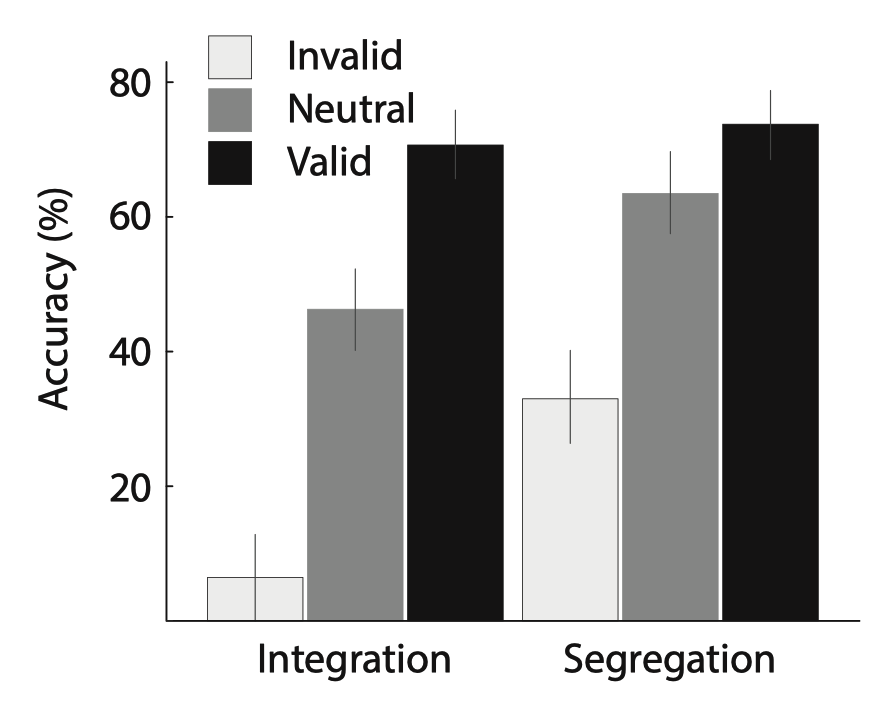
\includegraphics[height = 0.7 \textheight]{images/res1.png}
            \end{figure}
        \end{column}
        
        \begin{column}{0.45\textwidth}
    
        \only<2->{
            \small
            \begin{itemize}
                \item<2-> valid cues ($+$), invalid cues ($-$)
                \item<3-> greater effect of cues in the segregation task
                \item<4-> supported by eye-tracking:
                \begin{itemize}\footnotesize
                    \item[-] visual angle shifts towards the cue direction
                    \item[-] no significant differences between integration and segragation
                \end{itemize}
            \end{itemize}
            }
        
        \end{column}
        \end{columns}
    
\end{frame}

\begin{frame}{Result 2: Suitability of the Data to Measure $\alpha$ Frequency}
    \begin{columns}

        \begin{column}{0.5\textwidth}
            \begin{figure}\label{fig:res2}
            \centering
            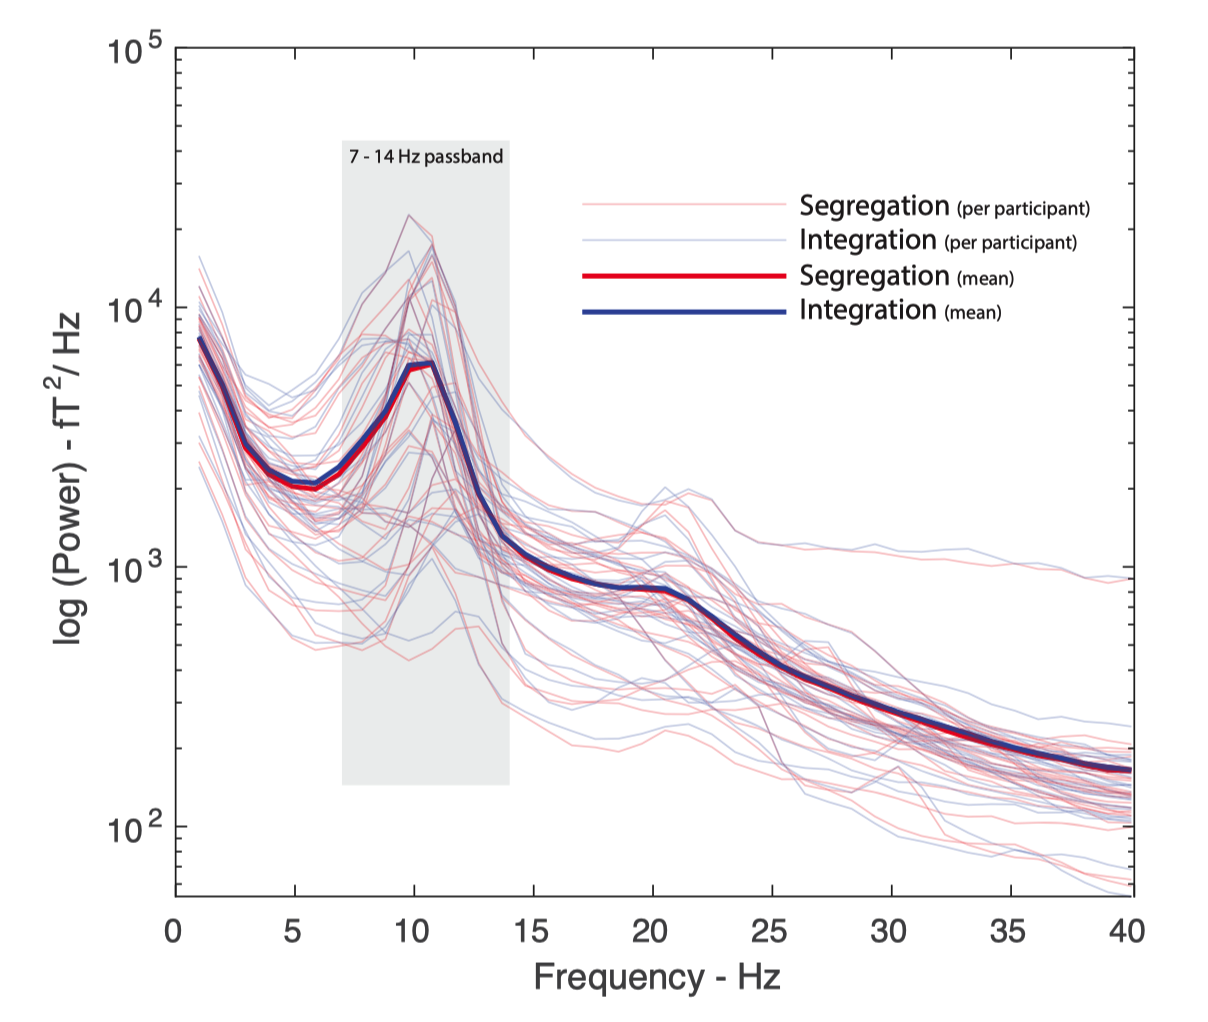
\includegraphics[height = 0.7 \textheight]{images/res2.png}
            \end{figure}
        \end{column}
        
        \begin{column}{0.45\textwidth}
    
        \only<2->{
            \small
            \begin{itemize}
                \item<2-> the analytic passband (7-14Hz) contains \textcolor{lightlavender}{\textbf{the peak}} {\footnotesize (In fact, the entire $\alpha$ bump for all participants)}
                \item<3-> No significant difference in \textcolor{lightlavender}{\textbf{power}} or slope of the \textcolor{lightlavender}{\textbf{1/f structure}} between segregation and integration
            \end{itemize}
            }
        
        \end{column}
        \end{columns}
    
\end{frame}

\begin{frame}{Result 3: $\alpha$ Rate Is Higher for Segregation Tasks}
    \begin{columns}

        \begin{column}{0.6\textwidth}
            \begin{figure}\label{fig:res3_1}
            \centering
            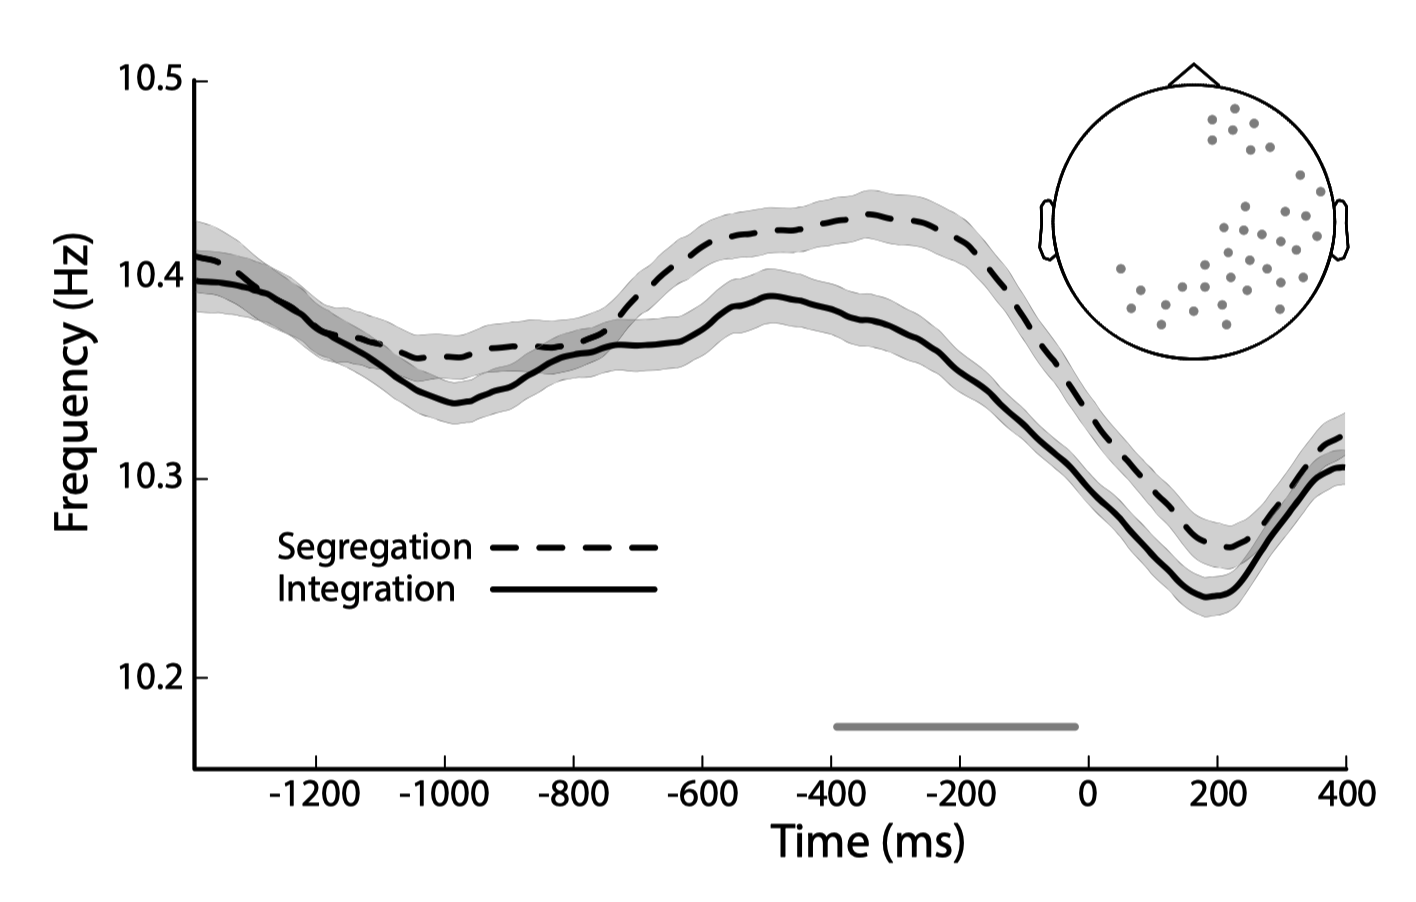
\includegraphics[height = 0.7 \textheight]{images/res3_1.png}
            \end{figure}
        \end{column}
        
        \begin{column}{0.35\textwidth}
    
        \only<2->{
            \small
            \begin{itemize}
                \item<2-> significantly higher $\alpha$ rate for \textcolor{lightlavender}{\textbf{segregation}} before 1st display {\footnotesize (t=0: the 1st display)}
                \item<3-> results are from instantaneous frequency analysis of \textcolor{lightlavender}{\textbf{neutral-cue}} trails
            \end{itemize}
            }
        
        \end{column}
        \end{columns}
    
\end{frame}

\begin{frame}{Result 3: $\alpha$ Rate Is Higher for Segregation Tasks, Source Analysis}
    \begin{columns}

        \begin{column}{0.6\textwidth}
            \begin{figure}\label{fig:res3_2}
            \centering
            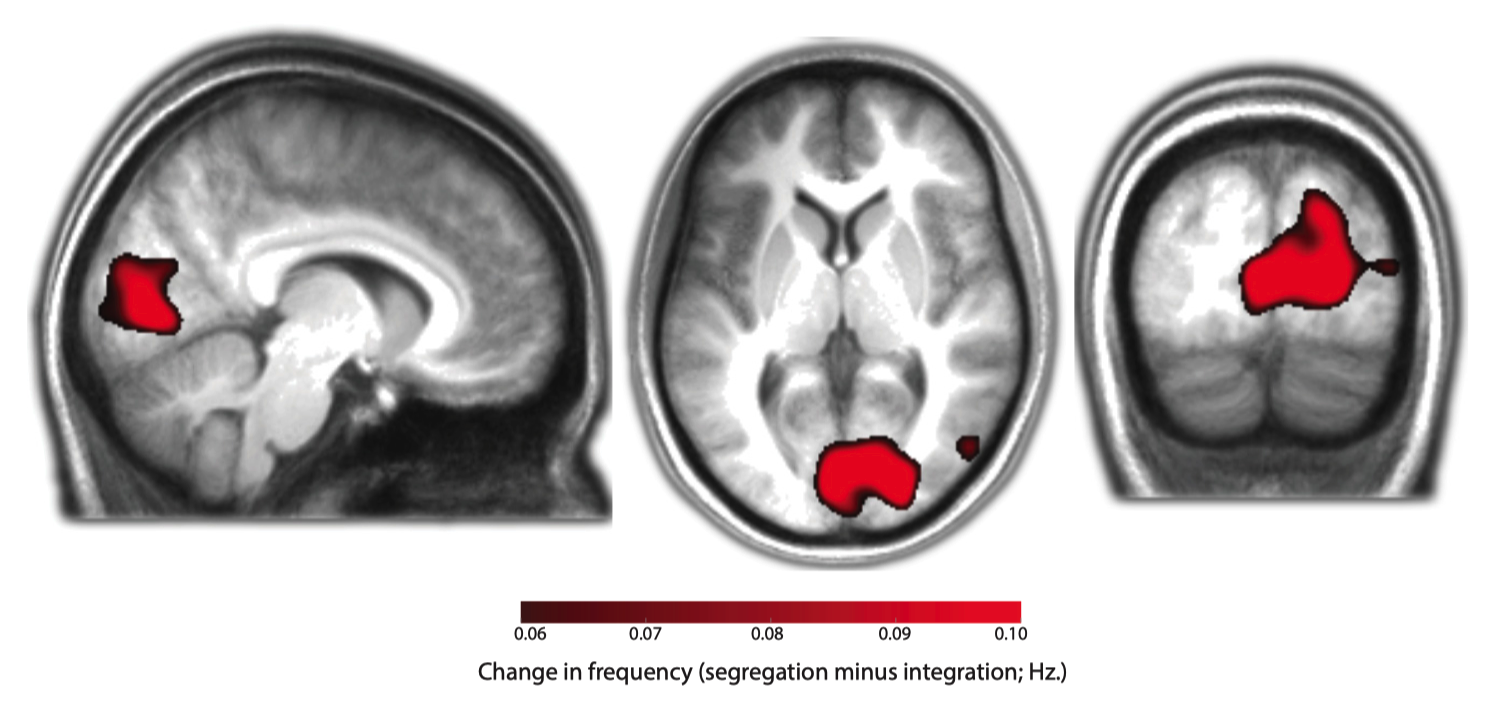
\includegraphics[height = 0.5 \textheight]{images/res3_2.png}
            \end{figure}
        \end{column}
        
        \begin{column}{0.35\textwidth}
    
        \only<2->{
            \small
            \begin{itemize}
                \item bilateral occipito-parietal cortex
                \item right lateralized frontal cortex
            \end{itemize}
            }
        \only<3->{
            \footnotesize
            replicate the observations of \citet{wutz2018frequency}
        }
        
        \end{column}
        \end{columns}
    
\end{frame}

\begin{frame}{Main Result: Lateral Analysis of $\alpha$ Frequency}
    \begin{columns}

        \begin{column}{0.45\textwidth}
            \begin{figure}\label{fig:res4}
            \centering
            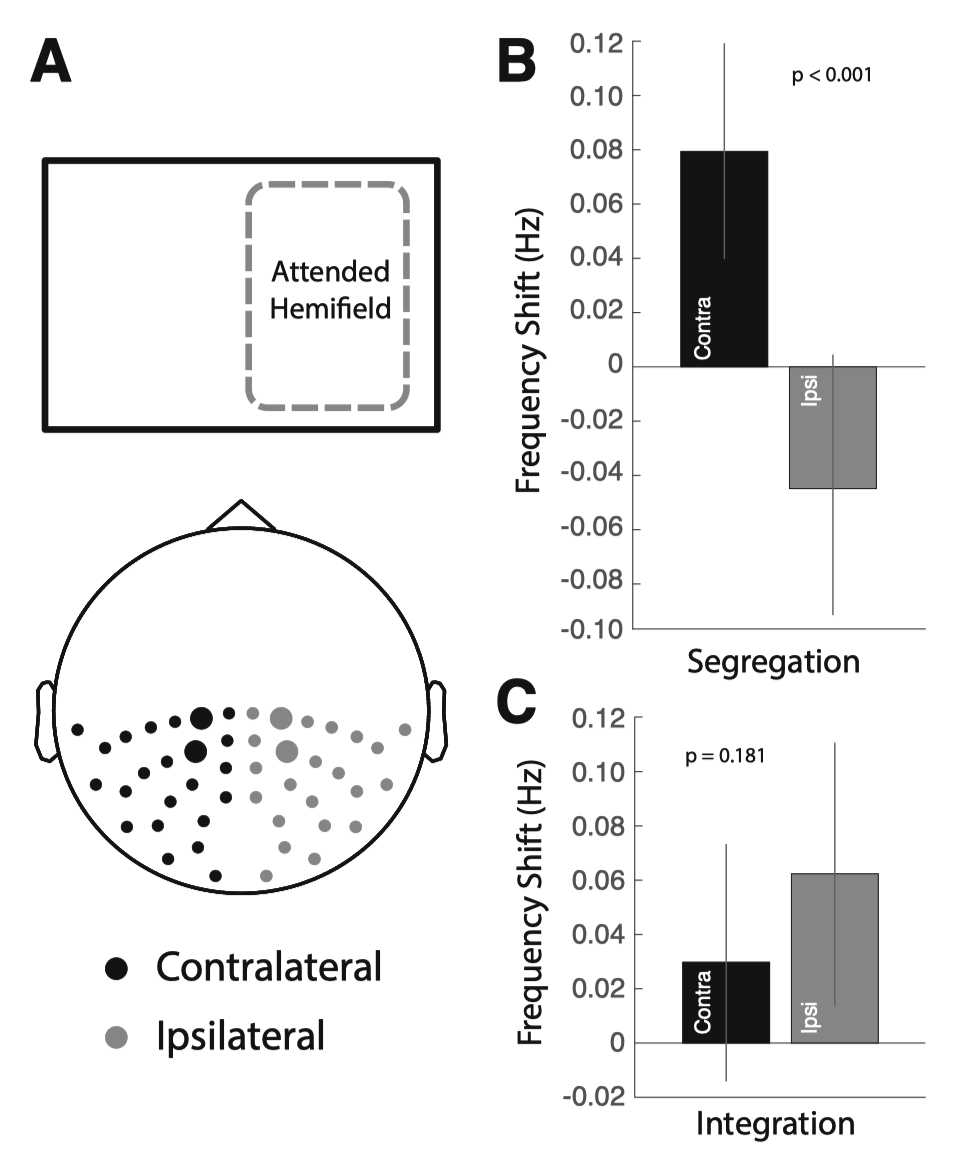
\includegraphics[height = 0.75 \textheight]{images/res4_1.png}
            \end{figure}
        \end{column}
        
        \begin{column}{0.55\textwidth}
    
        \only<2->{
            \small
            \begin{itemize}
                \item<2-> base: any retinotopic effect \textcolor{lightlavender}{\textbf{must}} emerge over \textcolor{lightlavender}{\textbf{posterior cortex}}
                \item<3-> results:
                \begin{itemize}
                    \item[-] segregation (faster $\alpha$ rate): contralateral \textcolor{lightlavender}{\textbf{faster}} than ipsilateral
                    \item[-] integration (slower $\alpha$ rate): contralateral \textcolor{lightlavender}{\textbf{slower}} than ipsilateral
                \end{itemize}
            \end{itemize}
            }
        
        \end{column}
        \end{columns}
    
\end{frame}

\begin{frame}{Main Result: Lateral Analysis of $\alpha$ Frequency}
 
    \begin{figure}\label{fig:res4_2}
    \centering
    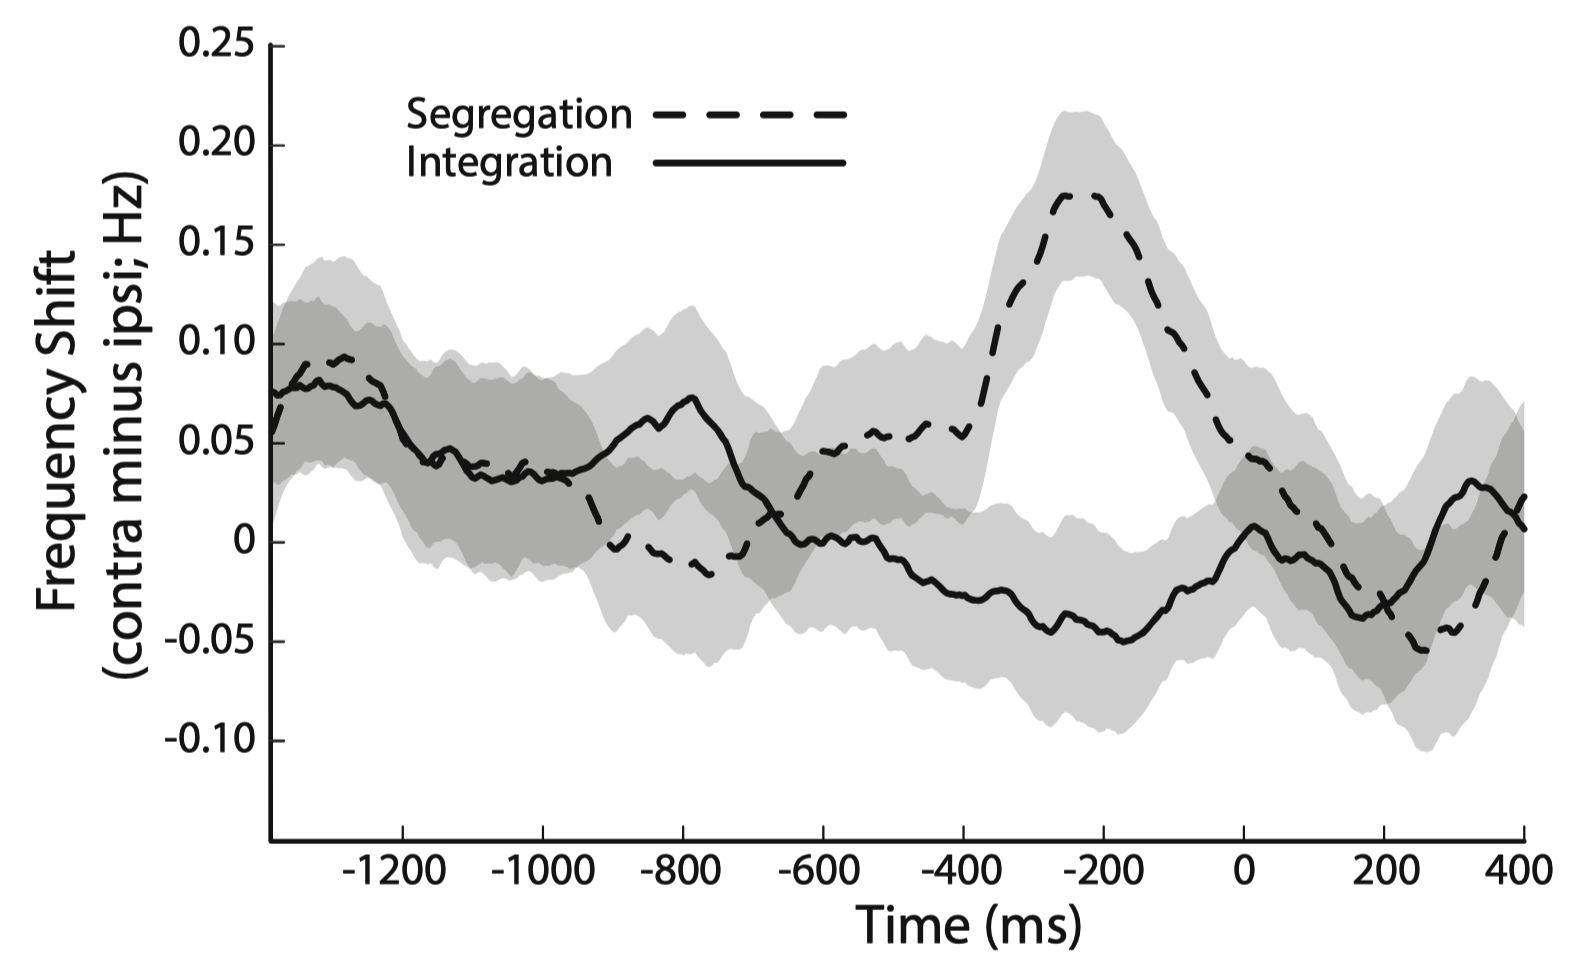
\includegraphics[height = 0.75 \textheight]{images/res4_2.png}
    \end{figure}
    
\end{frame}

\begin{frame}{Main Result: Ruling out the Effect of Lateral Oscillatory $\alpha$ Power}
    \begin{columns}

        \begin{column}{0.6\textwidth}
            \begin{figure}\label{fig:res5}
            \centering
            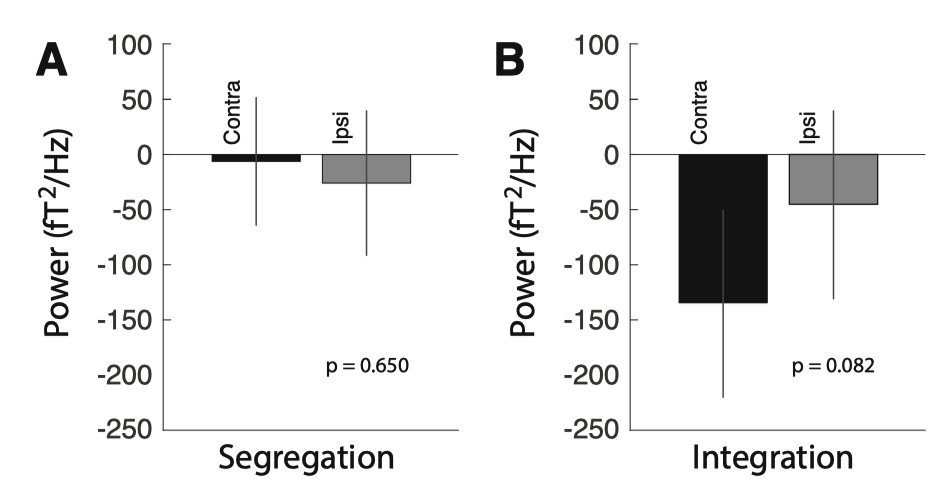
\includegraphics[height = 0.55 \textheight]{images/res5.png}
            \end{figure}
        \end{column}
        
        \begin{column}{0.35\textwidth}
    
        \only<2->{
            \small
            \begin{itemize}
                \item no significant differences in the lateral effect between segregation and integration
                \item no significant decrease in $\alpha$ power in contralateral hemisphere
            \end{itemize}
            }
        \only<3->{
            \footnotesize
            replicate the observations of \citet{capilla2014dissociated} that the decrease in $\alpha$ power is sourced to \textcolor{lightlavender}{\textbf{ventrolateral visual cortex}}
        }
        
        \end{column}
        \end{columns}
    
\end{frame}

\begin{frame}{Main Result: Lateral Analysis of $\alpha$ Frequency, Source Analysis}
    \begin{columns}

        \begin{column}{0.45\textwidth}
            \begin{figure}\label{fig:res6}
            \centering
            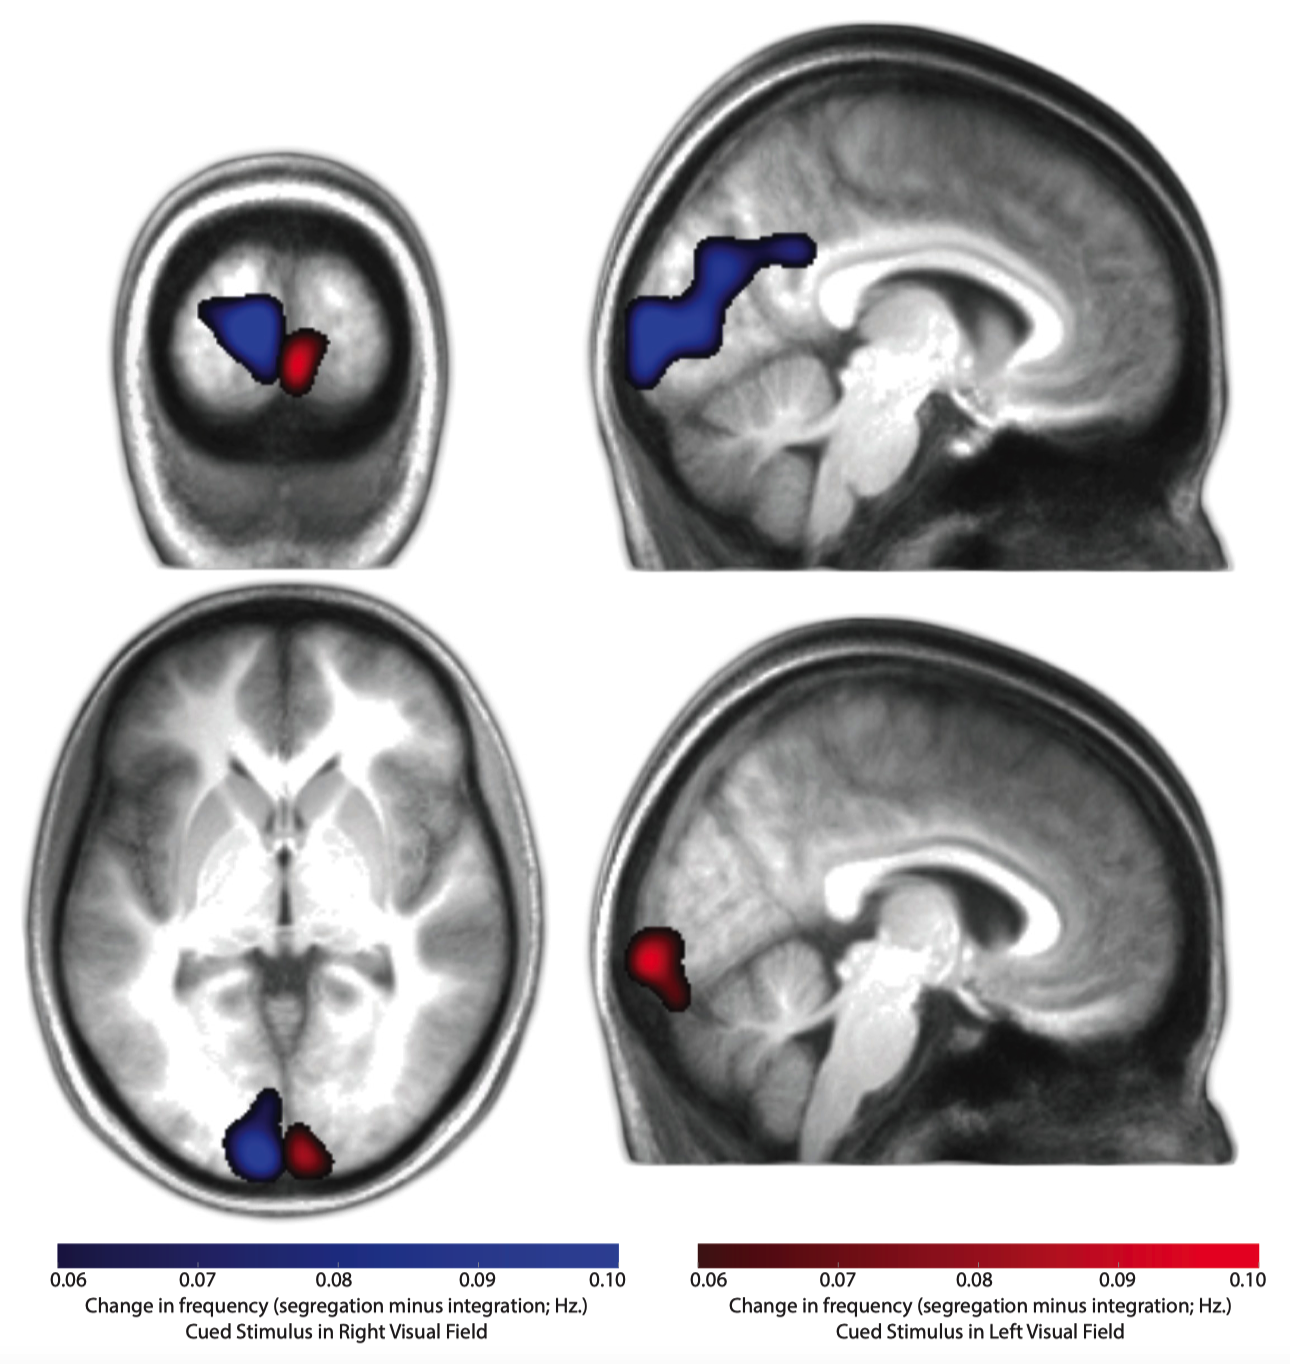
\includegraphics[height = 0.75 \textheight]{images/res6.png}
            \end{figure}
        \end{column}
        
        \begin{column}{0.55\textwidth}
    
        \only<2->{
            \small
            \begin{itemize}
                \item<2-> both clusters are located in \textcolor{lightlavender}{\textbf{early visual areas}} at the \textcolor{lightlavender}{\textbf{occipital}} pole
                \item<3-> note:
                \begin{itemize}
                    \item[-] \textcolor{blue}{\textbf{blue}}: stimuli in \textcolor{blue}{\textbf{right}} visual field
                    \item[-] \textcolor{red}{\textbf{red}}: stimuli in \textcolor{red}{\textbf{left}} visual field
                \end{itemize}
            \end{itemize}
            }
        
        \end{column}
        \end{columns}
    
\end{frame}